% % \part{优化模型}
% % \chapter{几何规划}


% \documentclass[UTF8]{ctexbook}

% \ctexset{
%     part/number = \chinese{part}
% }
% \usepackage{amsmath}% ams 数学公式
% \usepackage{mathtools}% ams 数学公式
% \usepackage{amsfonts}% ams 数学字体
% \usepackage{amssymb,latexsym}% ams 数学符号与LaTeX数学符号
% \usepackage{mathrsfs}% 花式符号
% \usepackage{ntheorem}%定理、定义、证明
%   \theoremstyle{nonumberplain}
%   \theoremheaderfont{\bfseries}
%   \theorembodyfont{\normalfont}
%   \theoremsymbol{$\square$}
%   \newtheorem{Proof}{\hskip 2em 证明}
%   \newtheorem{theorem}{\hspace{2em}定理}[chapter]
%   \newtheorem{definition}{\hspace{2em}定义}[chapter] % 如果没有章, 只有节, 把上面的[chapter]改成[section]
%   \newtheorem{axiom}[definition]{\hspace{2em}公理}
%   \newtheorem{lemma}[definition]{\hspace{2em}引理}
%   \newtheorem{proposition}[definition]{\hspace{2em}命题}
%   \newtheorem{corollary}[definition]{\hspace{2em}推论}
%   \newtheorem{remark}{\hspace{2em}注}[chapter] %类似地定义其他“题头”. 这里“注”的编号与定义、定理等是分开的

% \usepackage{enumerate}%itemiz环境。\begin{enumerate}[step 1]
% \usepackage{cite}%参考文献
%     \bibliographystyle{plain}
% \usepackage{extarrows}% 带参数的箭头
% \usepackage{hyperref}% 超链接
% %\usepackage[CJKbookmarks, colorlinks, bookmarksnumbered=true,pdfstartview=FitH,linkcolor=black,citecolor=black]{hyperref}%超链接的格式设置
% \hypersetup{
%     colorlinks=false,% 去掉超链接颜色
%     pdfborder=0 0 0% 取消超链接的边框
% }
% \usepackage{graphicx}% 图片管理
% \usepackage{caption}
% \usepackage{subcaption}%并排的图各有标题
% \graphicspath{{images/}}% 设置图片搜索路径
% \usepackage{float,varwidth}% 浮动体
% \usepackage{booktabs}% 三线表
% \usepackage{fancyhdr}% 页眉设置
% \usepackage{xcolor}% 颜色宏包
% \usepackage{colortbl}% 彩色表格
% \usepackage{listings}% 代码高亮
% \usepackage{caption}% 对标题进行控制,如让\caption标题的字体缩小一号,同时数字标签使用粗体可以用:\usepackage[font=small,labelfont=bf]{caption}
% \usepackage{xfrac,upgreek}%分别是行间公式如a/b的形式(将原来的命令\frac改成\sfrac)和希腊字体的宏包的
% \usepackage{mathtools}%lgathered和rgathered环境把公式向左向右对齐
% \usepackage{tabularx}%提供自动延伸的表列,(X列格式说明符),文字过长时可以自动转行
% \usepackage{longtable}%长表格
% \usepackage{enumitem}%enumerate宏包的升级
% \usepackage{harpoon}%数学公式的矢量
% \usepackage{bookmark}%目录的书签
% \usepackage{pifont}%给数字加上圈。然后在正文输入\ding{172}~\ding{211}得到相应数字,要是要①就输入:\ding{172}②就输:\ding{173}
% \renewcommand{\headwidth}{\textwidth}%图片并排,这个要列在所有宏包的后面
% \makeatletter
% \newcommand{\rmnum}[1]{\romannumeral #1}
% \newcommand{\Rmnum}[1]{\expandafter\@slowromancap\romannumeral #1@}
% \makeatother
% \definecolor{codegreen}{rgb}{0,0.6,0}
% \definecolor{codegray}{rgb}{0.5,0.5,0.5}
% \definecolor{codepurple}{rgb}{0.58,0,0.82}
% \definecolor{backcolour}{rgb}{0.95,0.95,0.92}
% \lstset{
%     commentstyle=\color{codegreen},
%     keywordstyle=\color{magenta},
%     numberstyle=\tiny\color{codegray},
%     stringstyle=\color{codepurple},
%     basicstyle=\footnotesize,
%     breakatwhitespace=false,% 断行只在空格处
%     breaklines=true,% 自动断行
%     captionpos=b,% 标题位置
%     keepspaces=true,
%     numbers=left,
%     numbersep=5pt,
%     showspaces=false,
%     showstringspaces=false,
%     showtabs=false,% 显示
%     tabsize=2% TAB 被当作两个空格
% }
% \topmargin=0pt\oddsidemargin=0pt\evensidemargin=0pt
% \textwidth=16.5cm\textheight=23cm\raggedbottom%我这么设置是为了缩小页边距,满足有的文字无法转行
% \pagestyle{headings}%页眉为章节标题,无页脚
% \setlength{\abovecaptionskip}{4pt}
% \setlength{\belowcaptionskip}{-8pt}%图片表格的前后距离设置
% \CTEXsetup[format={\zihao{-3}\raggedright\bfseries}]{section}%设置节的格式

% \begin{document}
% \part{优化模型}
\chapter{几何规划}
\section{问题的引入与分析}
    \par
    考虑如下优化问题
    \begin{align*}
    &\mathop{\max}\  x/y\\
    &s.t.  \left\{
    \begin{aligned}
    &2\leqslant x\leqslant 3\\
    &x^2+3y/z\leqslant \sqrt{y}\\
    &x/y=z^2\\
    &xyz>0
    \end{aligned}
        \right.
    \end{align*}
    其中:$x,y,z\in R$为决策变量。将上述问题转化为GP(几何规划)的标准形
    \begin{align*}
    &\mathop{\min}\  x^{-1}y\\
    &s.t.  \left\{
    \begin{aligned}
    &2x^{-1}\leqslant 1\\
    &\frac 13 x\leqslant 1\\
    &x^2y^{-1/2}+3y^{1/2}z^{-1}\leqslant 1\\
    &xy^{-1}z^{-2}=1
    \end{aligned}
    \right.
    \end{align*}
\section{模型规范化及其基础理论}
    \par
    几何规划GP的一般形式为
    \begin{align*}
    &\mathop{\min}\  f_0(x)\\
    &\begin{aligned}
    s.t.\quad &f_l(x)\leqslant 1\quad l\in I\\
    &x>0
    \end{aligned}
    \end{align*}
    其中:$x\in R^n$为决策变量,$I=\{1,2,\ldots,L\}$,$f_l(x)$如下
    \begin{align*}
    &f_l(x)=\mathop{\sum}\limits_{j=1}^{m_l}{\sigma}_{lj}c_{lj}\mathop{\prod}\limits_{i=1}^{n}x_i^{a_{lij}}
    \end{align*}
    $l\in I,{\sigma}_{lj}=\pm 1,c_{lj} > 0,a_{lij}$为任意给定的实数,$a_{lij}\in R$。
    \par
    几何规划GP最初由Zener于1961年提出,是非线性规划的一类分支。Zener毕业于哈佛大学,主攻物理。在后来的实践中,他发现许多工程设计问题均可归纳为一种特殊的形式GP:目标函数和约束函数$f_l(x)$为自变量$x$乘幂之代数和的形式。Richard Dufin主要从事于非线性对偶理论的研究,在发现Zener的工作后,与他一起从事这项研究。这种方法最初的发展使用了\underline{算数几何平均不等式},因此,Dufin称这种问题为几何规划。Dufin和Zener主要是讨论正系数的问题,也即正定式几何规划。1967年,Passy和Wilde提出了广义几何规划的伪对偶理论。再后来,Peterson提出一般无约束几何规划的对称对偶定理。70年代压缩方法在求解广义几何规划中很受欢迎。
    \subsection{几何规划解法介绍}
        \par
        正定式几何规划的局部极小点即为全局极小点,只需要对正定式几何规划进行变量替换:$x_i=e^i(i=1,2,\ldots,n)$,替换后的原正定式几何规划就等价转化为凸规划问题,原问题就等于凸区域上极小化一个凸函数,这种性质是正定式几何规划的一个非常重要的特征。正定式几何规划的主要解法有:\ding{172}割平面法;\ding{173}对偶方法;\ding{174}压缩法;\ding{175}在半无限线性规划基础上的另一种新的对偶方法。广义几何规划的主要解法有:对偶方法和两种压缩法等。
\section{正定式几何规划}
    \subsection{一般形式及对偶规划}
        \par
        下面,我们给出正定式几何规划(PGP)的一般形式
        \begin{align*}
        &\mathop{\min}\limits_{x}\  f_0(x)\\
        &\begin{aligned}
        s.t.\quad &f(x)\leqslant 1\quad l=\{1,2,\ldots,L\}\\
        &x \geqslant 0
        \end{aligned}
        \end{align*}
        其中:$x\in R^n$,$f_l(x)=\mathop{\sum}\limits_{j=1}^{m_l}c_{lj}\mathop{\prod}\limits_{i=1}^{n}x_i^{a_{lij}}$,$l=0,1,2,\ldots,L$。
        \par
        我们对PGP进行变量替换,令$y_i={\log}x_i$,从而将其变为凸规划:
        \begin{align*}
            f_l(x)&=\mathop{\sum}\limits_{i=1}^{m_l}c_{lj}\mathop{\prod}\limits_{i=1}^{n}(e^{y_i})^{a_{lij}}\\
            &=\mathop{\sum}\limits_{j=1}^{m_l}c_{lj}e^{a_{lj}^\mathrm{T} \cdot y}
        \end{align*}
        再令${\beta}_{lj}={\log}c_{lj}$,有
        \begin{align*}
            f_l(y)&=\mathop{\sum}\limits_{j=1}^{m_l}(e^{{\beta}_{lj}})\cdot e^{a_{lj}^\mathrm{T} \cdot y}\\
            &=\mathop{\sum}\limits_{j=1}^{m_l}e^{a_{lj}^\mathrm{T} \cdot y+{\beta}_{lj}}
        \end{align*}
            于是,原问题变为如下问题
        \begin{align*}
            &\mathop{\min}\limits_{y}\  f_0(y)\\
            &s.t.\quad f_l(y)\leqslant 1
            \end{align*}
        其中:$y$为优化变量,$f_l(y)=\mathop{\sum}\limits_{j=1}^{m_l}e^{a_{lj}^\mathrm{T} \cdot y+{\beta}_{lj}}$。对上式两边取对数,有
        \begin{align*}
            &\mathop{\min}\  {{\tilde{f}}_0(y)}={\log}\mathop{\sum}\limits_{j=1}^{m_l}e^{a_{0j}^\mathrm{T} \cdot y+{\beta}_j}\\
            &s.t.\quad {{\tilde{f}}_l(y)}={\log}\mathop{\sum}\limits_{j=1}^{m_l}e^{a_{lj}^\mathrm{T} y +{\beta}_{lj}}\leqslant 0\\
            &\qquad j=1,2,\ldots,L
        \end{align*}
        \par
        上述规划问题的目标函数和约束条件${{\tilde{f}}_l(y)}$均为凸函数,所以原PGP转化为凸形式的几何规划。下面讨论PGP的对偶问题。
        \par
        设一个$m_L$行$n$列的矩阵为正定式几何规划的指数矩阵。
        \begin{equation*}
        A=\begin{pmatrix}
        a_{011}&a_{012}&\dots&a_{01n}\\
        \vdots&\vdots&\ddots&\vdots\\
        a_{0m_01}&a_{0m_02}&\dots&a_{0m_0n}\\
        \vdots&\vdots&\ddots&\vdots\\
        a_{L11}&a_{L12}&\dots&a_{L1n}\\
        \vdots&\vdots&\ddots&\vdots\\
        a_{Lm_L1}&a_{Lm_L2}&\dots&a_{Lm_Ln}
        \end{pmatrix}_{m_L\times n}\\
        \end{equation*}
        其中:$a_{lij}$,$l = 0,1,\dots,L;i=1,2,\dots,n;j=1,2,\dots,m_l$,$n$为自变量$x$的维度,$m$是所有约束函数$f_l(x)$中的项数总和,即$m=m_0+m_1+\ldots +m_L$,此时,记$d(p)=\mathop{\prod}\limits_{l=0}^{L}\mathop{\prod}\limits_{j=1}^{m_l}(\frac{p_{l_0}c_{lj}}{p_{lj}})_{lj}^p$。
        \par
        称下面规划为PGP的对偶规划(SGP)
        \begin{align*}
        &\mathop{\max}\ {\ln} d(p)=\mathop{\sum}\limits_{l=0}^{L}\mathop{\sum}\limits_{j=1}^{m_l}{p}_{lj}\left({\ln}c_{lj}+\left( \mathop{\sum}\limits_{j=1}^{m_L}p_{lj} \right) -{\ln}p_{lj}\right)\\
        &s.t.\quad \left\{
        \begin{aligned}
        &\mathop{\sum}\limits_{j=1}^{m_0}p_{0j}=p_{00}=1\\
        &\mathop{\sum}\limits_{l=0}^{L}\mathop{\sum}\limits_{j=1}^{m_l}a_{lij}p_{lj}=0\quad i = 1,2,\ldots,n\\
        &p_{lj} > 0\quad l=0,1,\ldots,L;j=1,2,\ldots,m_l
        \end{aligned}
            \right.
        \end{align*}
        其中:$p_{l0}=\mathop{\sum}\limits_{j=1}^{m_l}{p}_{lj},l=0,1,\ldots,L$。
        \begin{theorem}
        如果一个几何规划(不包含等式约束)存在极小值,则有
        \par
        \ding{172}对偶问题的极大值存在;
        \par
        \ding{173}$d(p^*)=f_0(x^*)$,其中$p^*,x^*$为最优点;
        \par
        \ding{174}在最优点处,原变量与对偶变量的关系为:
        \begin{align*}
        &c_{0j}\mathop{\prod}\limits_{i=1}^{n}(x^*_i)_{0ij}^a=p_{0j}^*f_0(x^*)x_i^*\\
        & j=1,2,\ldots,m_0\\
        &c_{lj}\mathop{\prod}\limits_{i=1}^{n}(x^*_i)_{lij}^a=\frac{p_{lj}^*}{p_{l0}^*}\\
        &p_{lj}^*(1-f_l(x^*))=0
        \end{align*}
        其中:$l=1,2,\ldots,L$。
        \end{theorem}
        \par
        此定理不仅告诉我们原问题的最小值等于对偶问题的最大值,而且只要求出对偶问题的最优点和最优值通过上面的关系\ding{172} - \ding{174}即可求出原问题的最小点。从形式上看,上面的关系\ding{174}为未知数的非线性方程组,取对数之后,就得到以${\ln}x_i$为未知数的线性方程组,即
        \begin{align*}
        &\mathop{\sum}\limits_{i=1}^{n}a_{0ij}{\ln}x_i^*=\ln \frac{p_{0j}^*d(p^*)}{c_{0j}}\quad j=1,2,\ldots,m_0\\
        &\mathop{\sum}\limits_{i=1}^{n}a_{lij}{\ln}x_i^*=\ln \frac{p_{ij}^*}{p_{l0}^*c_{lj}} \quad l=0,1,\ldots,L;j=1,2,\ldots,m_l
        \end{align*}
        \par
        此方程的个数为$\mathop{\sum}\limits_{l=0}^{m_L}=m$,未知量的个数为$n$。根据线性方程组的理论,可以解出${\ln}x_i^*(i=1,2,\ldots,n)$,从而得到$x^*=(x_1^*,x_2^*,\ldots,x_n^*)$。
        \par
        由于对偶规划(SGD)是一凹规划,因此,许多算法都是基于它来求解原PGP的,但是目标函数$d(p)$在$p_{lj}=0$上是不可微的。尽管这样,我们仍能发现对偶规划(SGD)有非常重要的特征,其约束函数是线性的,而且目标函数$d(p)$是一凹函数。Beck提出一种改进的单纯形算法来求解对偶规划(SGD)。Alegandre充分利用了对偶规划的结构及其线性约束的特征,并为了克服不可微的缺陷,对所有变量增加严格正的下界约束,从而提出一种基于对偶的有效求解算法。
        \par
        在求解SGD时,需要定义一个困难度
        \begin{align*}
        d=m-n-1=\mathop{\sum}\limits_{l=0}^{l}m_{l}-n-1
        \end{align*}
        困难度用来衡量几何规划求解难度的一个重要指标。一般来说,困难度越大,求解越困难。
    \subsection{最优化方法}
        \subsubsection{信赖域内点算法}
            \par
            我们将SGD写为一般规划形式
            \begin{align*}
            &\mathop{\min}\limits_{x\in R^n}\  f(x)\\
            &s.t.\quad x\in G
            \end{align*}
            其中:
            \begin{align*}
            &f(x)=C^\mathrm{T} x+\mathop{\sum}\limits_{i=1}^{n}x_i{\ln}x_i-\mathop{\sum}\limits_{l=0}^{L}e_l^\mathrm{T} x{\ln}e_l^\mathrm{T} x\overset{\Delta}{=}-{\ln}d(P)\\
            &G=\{x|Ax=b,x>0\}\\
            &x=(x_1,x_2,\cdots,x_n)^\mathrm{T} \triangleq P = (P_{01},P_{0m_0},\cdots,P_{L_1},\cdots,P_{Lm_L})^\mathrm{T} \\
            &C=(c_1,c_2,\cdots,c_n)^\mathrm{T} \triangleq  -({\ln}C_{01},{\ln}C_{0m_0},\cdots,{\ln}C_{L_1},\cdots,{\ln}C_{Lm_L})^\mathrm{T} \\
            &b=(1,0,0,\cdots,0)^\mathrm{T} \in R^m,n=\mathop{\sum}\limits_{l=0}^{L} m_l
            \end{align*}
            $e_l$为从第$1+\sum_{k=0}^{l-1}m_k$位分量到第$\sum_{k=0}^l m_k$位分量(共$m_l$个分量)为1,其余分量为0的$n$维列向量。
            令$A$为
            \begin{equation*}
            A =
            \begin{bmatrix}
            \begin{smallmatrix}
            1 & \dots & 1&\dots &0 &\dots& 0& \dots &0&\dots &0\\
            a_{011} &\dots & a_{01m_0}&\dots &a_{111} &\dots& a_{11m_1}& \dots &a_{L11}&\dots &a_{L1m_L}\\
            a_{021} &\dots & a_{02m_0}&\dots &a_{121} &\dots& a_{12m_1}& \dots &a_{L21}&\dots &a_{L2m_L}\\
            \vdots& \ddots & \vdots & \ddots & \vdots & \ddots & \vdots & \ddots & \vdots & \ddots & \vdots \\
            a_{0m-11} &\dots & a_{0m-1m_0}&\dots &a_{1m-11} &\dots& a_{1m-1m_1}& \dots &a_{Lm-11}&\dots &a_{Lm-1m_L}
            \end{smallmatrix}
            \end{bmatrix}
            \end{equation*}
            则
            \begin{equation*}
            \begin{split}
            g(x)=-\nabla f(x)&=-[C+({\ln}(x_1/e_0^\mathrm{T} x),\cdots,{\ln}(x_{m_0}/e_0^\mathrm{T} x),{\ln}(x_{m_0+1}/e_1^\mathrm{T} x),\cdots,{\ln}(x_{m_0+m_1}/e_1^\mathrm{T} x),\\
            &\quad \cdots,{\ln}(x_{m_0+m_1}/e_1^\mathrm{T} x),\cdots,{\ln}(x_{n-m_L+1}/e_L^\mathrm{T} x))]^\mathrm{T}
            \end{split}
            \end{equation*}
            \begin{align*}
           {\nabla}^2 f(x)=\begin{bmatrix}
           \frac{1}{x_1}&{}&{}&{}\\
           {}&\frac{1}{x_2}&{}&{}\\
           {}&{}&\ddots&{}\\
           {}&{}&{}&\frac{1}{x_n}
           \end{bmatrix}-\begin{bmatrix}
           \frac{D_0}{e_0^\mathrm{T} x}&{}&{}&{}\\
           {}&\frac{D_1}{e_1^\mathrm{T} x}&{}&{}\\
           {}&{}&\ddots&{}\\
           {}&{}&{}&\frac{D_L}{e_L^\mathrm{T} x}
           \end{bmatrix}
            \end{align*}
            其中:$D_l$为全1的$m_l\times m_l$方阵。
            \par
            我们已经知道,在最优解$x^*=p^*$之后,只需解方程组即可求解原PDP的解($t^*$),这里为了防止混淆,我们都用$t^*$来作为原问题的决策变量。
            \begin{align}
            \label{几何规划的决策变量}
            &\mathop{\sum}\limits_{i=1}^{n}a_{0ij}{\ln}t_i^*={\ln}\left( \frac{p_{0j}^*d(p^*)}{c_{0j}} \right) \quad j=1,2,\ldots,m_0\\
            &\mathop{\sum}\limits_{i=1}^{n}a_{lij}{\ln}t_i^*={\ln}\left( \frac{p_{1j}^*}{p_{0l}^*/c_{lj}} \right)  \quad l=0,1,\ldots,L;j=1,2,\ldots,m_l
            \end{align}
            其中:$p_{l0}^*=\mathop{\sum}\limits_{j=1}^{m_l}p_{lj}^*\quad l=0,1,\ldots,L$。
            解得${\ln}t_i^*$即为SGP的最优解$t^*$。
            \par
            引入线性约束内部可微凸规划的信赖域解法。
            假设1:SGP有最优解$x^*=p^*$;
            假设2:$rank(A)=m$,即A的行向量组线性无关。
            \par
            首先,我们定义如下矩阵
            \begin{align*}
             H=H(x)=\begin{bmatrix}
              {\Delta}_0(x)&{}&{}&{}\\
             {}&{\Delta}_1(x)&{}&{}\\
             {}&{}&\ddots&{}\\
             {}&{}&{}&{\Delta}_l(x)
             \end{bmatrix}-\begin{bmatrix}
             \frac{D_0}{\sigma+e_0^\mathrm{T} x}&{}&{}&{}\\
             {}&\frac{D_1}{\sigma+e_1^\mathrm{T} x}&{}&{}\\
             {}&{}&\ddots&{}\\
             {}&{}&{}&\frac{D_L}{\sigma+e_L^\mathrm{T} x}
             \end{bmatrix}
              \end{align*}
              其中:
              \begin{align*}
             \begin{bmatrix}
              {\Delta}_0(x)&{}&{}&{}\\
             {}&{\Delta}_1(x)&{}&{}\\
             {}&{}&\ddots&{}\\
             {}&{}&{}&{\Delta}_l(x)
             \end{bmatrix}=\begin{bmatrix}
             \frac{1}{x_1}&{}&{}&{}\\
             {}&\frac{1}{x_2}&{}&{}\\
             {}&{}&\ddots&{}\\
             {}&{}&{}&\frac{1}{x_n}
             \end{bmatrix}
              \end{align*}
            ${\Delta}_l(x)$为$m_l$阶对角矩阵,$1>\sigma >0$为一常数,记$H_k=H(x^k)$。
            \begin{lemma}[1]
            $H=H(x)$为正定对称矩阵。
            \end{lemma}
            \begin{lemma}[2]
            原问题的一阶稳定条件(KKT条件):$\exists x^*\in R^n,{\lambda}^*\in R^{m+1},{\mu}^*\in R^n$满足:
            \begin{align*}
                &{\nabla} f(x^*)+A^\mathrm{T} {\lambda}^*=0\\
                &Ax^*=b\\
                &u_i^*x_i^* = 0\quad i=1,2,\cdots,n\\
                &x^*\geqslant 0,u^*\geqslant 0
                \end{align*}
            \end{lemma}
            \par
            定义$F=\{x\in R^n|Ax=b,x\geqslant 0\}$,$\hat{F}=\{x\in R^n|Ax^*=b,x > 0\}$。设$F$有界,$\hat{F}$非空,用$x^k$表示第$k$次求出的点。求试探步$d^k$,若接受,则$x^{k+1}=x^k+d^k$。记$X_k=diag(x^k)$,所有范数为$L_2$范数,$f_k=f(x^k),\nabla f_k=\nabla f(x^k)$。
            \par
            算法步骤:\\
            \textbf{step1.}初始化。
            \par
            $x_0\in \hat{F},\delta \in (0,1),\eta \in (0,1),0<{\sigma}_1<{\sigma}_2<1$,置$k:=0$.\\
            \textbf{step2.}求出$H_0$,$\Delta k\in(\delta,1/\delta)^0$。\\
            \textbf{step3.}求下面问题的全局$d^k$。
            \begin{align*}
            &\mathop{\min} \  {\psi}_k(d)={\nabla}f_k^\mathrm{T} d+\frac 12 d^\mathrm{T} H_kd\\
            &s.t.\quad \left\{
            \begin{aligned}
            &Ad=0 \\
            &\|X_k^{-1}d\|\leqslant {\Delta}_k
            \end{aligned}
                \right.
            \end{align*}
            使$x^k+d^k>0$。\\
            \textbf{step4.}如果${\psi}_k(d^k)={\psi}_k(0)=0$,停止计算。\\
            \textbf{step5.}做下降性测试,计算
            \begin{align*}
                r_k=\frac{f(x^k)-f(x^k+d^k)}{-{\psi}_k(d^k)}
            \end{align*}
            \textbf{step6.}若$r_k<\eta$,取${\Delta}_k\in ({\sigma}_1\|X_k^{-1}d^k\|,{\sigma}_2{\Delta}_k)$,返回step3,重新求$d^k$;否则$\Delta k = \Delta k;x^{k-1} = x^k+d^k$。\\
            \textbf{step7.}计算$f_{k+1}$,$\nabla f_{k+1}$,置$k:=k+1$,返回step2。
            \par
            下面给出上述算法的全局收敛性。\\
            假设1:$\exists x_0 \in \hat{F}$,且水平集$L=\{x\in F|f(x)\leqslant f(x^*)\}$是紧集;\\
            假设2:$\{H_k\}$一致有界;\\
            假设3:$\forall I\subset N,{\lambda}\in R^{m+1},u\in R^n$
            \begin{align*}
            & \nabla f(x)+A^\mathrm{T} \lambda -u =  0\\
            & Ax = b\\
            & x_I = 0\\
            & u_i = 0\\
            & i \notin I
            \end{align*}
            若有界,则只有孤立解。
            \begin{lemma}
            ${\psi}_k(d^k)=\psi(0)=0$,当且仅当$x^k$是问题P的稳定点。
            \end{lemma}
            \begin{lemma}
            算法产生的$x^k$如果不是问题P的稳定点,则存在可行下降方向$d\neq 0$,也即存在有界数$\lambda$,有$d^\mathrm{T} \nabla f_k<0,x^k+\lambda d\geqslant 0,d^\mathrm{T} \nabla f_k<0$。
            \end{lemma}
            \begin{lemma}
            算法产生的序列$\{x^k\}$有上界。
            \end{lemma}
            \begin{theorem}
            算法是有限的。
            \end{theorem}
            \begin{theorem}
            $x$为问题P的KKT点,则$x$为问题P的最优解。
            \end{theorem}
            \begin{theorem}
            $\{x^k\}$由算法产生,若有限步终止于$x^L$,则$x^k$为问题P的最优解;$\{x^k\}$的任一聚点$\bar{x}$为P的KKT点即最优解。
            \end{theorem}
        \subsubsection{广义梯度投影内点算法}
            \begin{lemma}
            $\forall x \in G,X=diag(x),A=(a_0,a_1,\cdots,a_{m-1})^\mathrm{T} $,其中$a_j(j=0,1,\ldots,m-1)$为$A$的行向量,则矩阵$AXXA^\mathrm{T} $是一对正定矩阵。
            \end{lemma}
            \par
            算法步骤:\\
            \textbf{step1.}初始化。
            \par
            $x_0\in G,{\sigma}_1>1,<{\sigma}_2>0$,置$k:=0$.\\
            \textbf{step2.}求$g(x^k)=-\nabla f(x^k)$,$B_k,P_k,\mu(x^k)$。
            \begin{align*}
                &B_{k}=B(x^k)=(AX_kX_kA^\mathrm{T} )^{-1}AX_k\\
                &P(x^k)=X_kX_k-X_kAB(x^k)\\
                &\mu (x^k) =({\mu}_0(x^L),{\mu}_1(x^L),\ldots,{\mu}_{m-1}(x^L))=B(x^k)X_kg(x^k)
                \end{align*}
            \textbf{step3.}求$s^k=P(X^k)=X_kg(x^k)$。
            \begin{align*}
                &{\rho}^k=\frac{|g(x^k)^\mathrm{T} D_ks^k|}{{\sigma}_1|\mu (x^l)^\mathrm{T} w|+{\sigma}_2}
                \end{align*}
                其中:$w=  (-1,-1,\dots,-1)^\mathrm{T} \in R^m$。\\
            \textbf{step4.}求$d^k=s^k+{\rho}^kp_ks^k$。\\
            \textbf{step5.}如果$g(x^k)^\mathrm{T} X_kd^k=0$,则$x^k$为问题P的KKT点,否则转到step6。\\
            \textbf{step6.}取$x_{k+1}=X_k(e+{\lambda}_kd^k)\in G$,其中$e=(1,1,\cdots)^\mathrm{T} \in R^n$,${\lambda}_k$为搜索步长,置$k:=k+1$返回step2。
            \par
            下面给出上述算法的全局收敛性:
            \par
            (1)算法有限步终止于问题P的某一KKT点,$x^k$也即最优点;
            \par
            (2)算法产生一无穷序列$\{x^k\}$,记$x^*$为其聚点,若$x^*>0$,且$\nabla f(x)$在G上关于$\{x^k\}$一致连续,则$x^*$为问题P的KKT点,也即最优点。
\section{广义几何规划}
    \par
    广义几何规划的一般形式为
    \begin{align*}
        &\mathop{\min} \  f_0(x)\\
        &s.t.\quad \left\{
        \begin{aligned}
        &f(x) \leqslant a_l\quad l=1,2,\ldots,L \\
        &x>0
        \end{aligned}
            \right.
        \end{align*}
        其中:$x \in R^n$,$f_l(x)=\mathop{\sum}\limits_{j=1}^{m_L}{\sigma}_{lj}c_{lj}\mathop{\prod}\limits_{i=1}^{n}x_i^{a_{lij}},l=0,1,\ldots,L$。
        ${\sigma}_{lj}=\pm 1$至少有一个是负的,$a_l=\pm 1$,$c_{lj}>0,l=0,1,\ldots,m_L$,$a_{lij}$为任一实数。
        \par
        广义几何规划的对偶形式为
        \begin{align}
        \label{广义几何规划的对偶形式1}
        &\mathop{\max} \  d(P)=a_0\left[\mathop{\prod}\limits_{l=0}^{L}\mathop{\prod}\limits_{j=1}^{m_l} \left( \frac{p_{l0}c_{lj}}{p_{lj}} \right) ^{{\sigma}_{lj}p_{lj}}\right]^{a_0}\\
        &s.t.\quad \left\{
        \begin{aligned}
        &\mathop{\sum}\limits_{l=1}^{m_0} {\sigma}_{0j}p_{0j}=a_0\\
        &\mathop{\sum}\limits_{l=0}^{L}\mathop{\sum}\limits_{j=1}^{m_l}{\sigma}_{lj}a_{lij}p_{lj}=0\\
        &p_{lj}\geqslant 0,i=1,2,\cdots,n
        \end{aligned}
        \right.
        \end{align}
        其中,规定
        \begin{align*}
        \mathop{\lim}\limits_{p_{lj}\to 0} \left(\frac{p_{l0}c_{lj}}{p_{lj}}\right)^{{\sigma}_{lj}p_{lj}} =1
        \end{align*}
        L个线性不等式约束
        \begin{align}
            \label{广义几何规划的对偶形式2}
        p_{l0}=a_l\mathop{\sum}\limits_{j=1}^{m_l}{{\sigma}_{lj}p_{lj}} \geqslant 0\quad l=1,2,\ldots,L
        \end{align}
        其中:$p_{00}=1$,
        \begin{align*}
        &a_0=\left\{
        \begin{aligned}
        &1\quad f_0(x^*)>0\\
        &-1\quad f_0(x^*)<0
                \end{aligned}
            \right.
        \end{align*}
        \begin{theorem}
        设有$m=\mathop{\sum}\limits_{l=0}^{L}m_l$个对偶变量$p_{lj}(l=0,1,\ldots,L;j=1,2,\ldots,m_L)$满足上述约束条件,$x^*$是原问题的最小点,则对$f_0(x)$的每个局部极小点$x^0$,存在一个对偶变量$p^0$满足式(\ref{广义几何规划的对偶形式1})(\ref{广义几何规划的对偶形式2})使得$d(p^0)=f_0(x^*)$,并且原有变量$x^0$与对偶变量$p^0$之间有如下关系:
        \begin{align*}
        &c_{0j}\mathop{\prod}\limits_{i=1}^{n}{x_i}^{a_{0ij}}=p_{0j}f_{0}(x^0)\quad j=1,2,\ldots,m_0\\
        &c_{lj}\mathop{\prod}\limits_{i=1}^{n}{x_i}^{a_{0ij}}=\frac{p_{lj}}{p_{l0}} \quad l=1,2,\ldots,L;j=1,2,\ldots,m_L
        \end{align*}
        以及
        \begin{align*}
        p_{lj}^0(1-f_l(x^0))=0 \quad l=1,2,\ldots,L;j=1,2,\ldots,m_l
        \end{align*}
        \end{theorem}
        \par
        下面,给出此问题的几点说明:\par
        \ding{172}$f(x)\geqslant d(P)$不一定成立。\par
        \ding{173}对于每一个$f(x)$的局部极小点$x^0$,必存在$p^0$使得$f(x^0)=d(p^0)$,$x^0$并非总体极小。
        \par
        \ding{174}当困难度为0时,由对偶约束确定唯一$p^0$与$d(p^0)$,又可确定$x^0$,可以证明原问题有极小点时,$x^0$即为极小点,$f(x^0)$即为极小值。
        \par
        \ding{175}由于事先不知道原问题(P)的极小点,$a_0$的取值带的符号难定,不过定错了也没关系,若$a_0$取错,所有对偶变量全为负值,与要求不符,就可以纠正$a_0$的值,再重新计算。
    \subsection{最优化算法}
        \par
        考虑不等式约束下的广义几何规划(GPE)
        \begin{align*}
            &\mathop{\min}\  f_0(t)\\
            &s.t.\quad f_l(t)\leqslant 0\quad l=1,2,\ldots,L
            \end{align*}
        其中:$t\in R^n$,
        \begin{align*}
        &f_l(t)=\mathop{\sum}\limits_{j=1}^{m_L}c_{lj}\mathop{\prod}\limits_{i=1}^{n}{t_i}^{a_{lij}}\\
        &\quad l=1,2,\ldots,L;j=1,2,\ldots,m_l,i=1,2,\ldots,n
        \end{align*}
        $c_{lj}$和$a_{lij}$为任意实数。
        \par
        令$x_i={\ln}{} t_i$,则GPE转化为如下等价形式$GPE_1$:
        \begin{align*}
        &\mathop{\min}\ C_0(x)=\mathop{\sum}\limits_{j=1}^{m_0}c_{0j}e^{\mathop{\sum}\limits_{i=1}^{n}a_{0ij}x_i}\\
        &s.t.\quad C_i(x)=\mathop{\sum}\limits_{j=1}^{m_l}c_{lj}e^{\mathop{\sum}\limits_{i=1}^{n}a_{lij}x_i}\leqslant 0\qquad l=1,2,\ldots,L
        \end{align*}
        \par
        将上式写为向量形式$GPE_2$,记$e^x=(e^{x_1},e^{x_2},\cdots,e^{x_n})^\mathrm{T} $,$A_l^\mathrm{T} =(a_{lij})_{n\times m_l}$,$b_l=(b_{l_1},b_{l_2},\cdots,b_{l_{m_l}})^\mathrm{T} $,$l=1,2,\ldots,L;j=1,2,\ldots,m_L,i=1,2,\ldots,n$,有
        \begin{align*}
        &\mathop{\min}\ C_0(x)=c_0^\mathrm{T} e^{A_0x}\\
        &s.t.\quad C_l(x)=c_{l}^\mathrm{T} e^{A_lx}\leqslant 0\qquad l=1,2,\ldots,L
        \end{align*}
        \par
        \underline{构造无约束优化问题}。设上面GPE的拉格朗日函数为
        \begin{align*}
        L(x,\lambda)=C_0(x)+\mathop{\sum}\limits_{l=1}^{L}{\lambda}_lC_l(x)
        \end{align*}
        记$\lambda=({\lambda}_l,{\lambda}_2,\cdots,{\lambda}_L)^\mathrm{T} $,$C(x)=(C_1(x),C_2(x),\cdots,C_L(x))^\mathrm{T} $。
        \par
        引入拉格朗日变量$Z_l$,将$GPE_2$中的不等式约束变为等式约束。
        \begin{align*}
        C_L(x)+Z_l^2=0\quad l=1,2,\cdots,L
        \end{align*}
        考虑$C_0(x)$在这组等式约束下的增广拉格朗日函数
        \begin{align*}
        \bar{L}(x,\lambda,z,\sigma)=C_0(x)+\mathop{\sum}\limits_{l=1}^{L}{\lambda}_l(C_l(x)+Z_l^2)+\frac{\sigma}{l}+\mathop{\sum}\limits_{l=1}^{L}(C_L(x)+Z_l^2)^2
        \end{align*}
        其中:$\sigma>0$为罚权重。
        为消去$Z_l$将$\bar{L}$关于$z$求极小,即令${\nabla}_z\bar{L}(x,\lambda,z,\sigma)=0$,得$Z_l({\lambda}_l+{\sigma}_l(C_l(x)+Z_l^2))=0,l=1,2,\cdots,L$。若${\sigma}_lC_l(x)+{\lambda}_l\leqslant 0$,则$Z_l^2=-\frac{{\lambda}_k}{{\sigma}_l}-C_l(x)$,否则$Z_l=0$。因此,$Z_l^2=-\frac{1}{{\sigma}_l}{\max}(0,-{\lambda}_l-{\sigma}_lC_l(x)),l=1,2,\cdots,L$。
        从而可得问题$GPE_2$的拉格朗日函数为
        \begin{align*}
        {L}(x,\lambda,\sigma)=C_0(x)+\frac{1}{2{\sigma}}\mathop{\sum}\limits_{l=1}^{L}\{[{\max}(0,{\sigma}C_l(x)+{\lambda}_l)]^2-{\lambda}_l \}
        \end{align*}
        之后,确定搜索方向$d_k$和步长${\alpha}_k$即可确定算法\footnote{几何规划问题的算法研究-晋香莲P16}。
        % \textcolor[rgb]{1 0 0}{todo:引入“”}
\section{MATLAB应用实例}
    \par
    悬梁臂的设计示意图如图(\ref{fig:悬梁臂示意图})所示
        \begin{figure}[H]
        \centering
        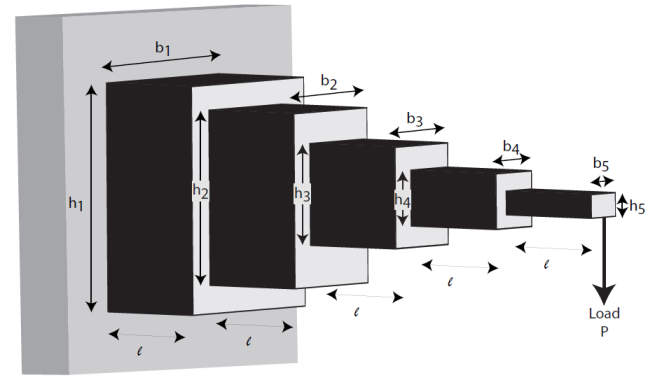
\includegraphics[height=4cm]{images/hanging_beam.jpg}
        \caption{悬梁臂示意图}
        \label{fig:悬梁臂示意图}
        \end{figure}
    \par
    设悬梁臂共有$N$块组成,第$i$块的长为$l$,宽为$w_i$,高为$h_i$(各块长均为$L$)。在悬梁臂末端悬挂重物$F$,要求设计各臂块$i$的$h_i,w_i$,来使悬梁臂总体体积$V$最小。当然,悬梁臂要满足一定的约束条件:
    \par
    \ding{172}边界约束
        \begin{align*}
            w_{\min}\leqslant w_i\leqslant w_{\max},\quad h_{\min}\leqslant h_i\leqslant h_{\max},\quad i=1,2,\cdots,N
        \end{align*}
    \par
    \ding{173}长宽约束
        \begin{align*}
            s_{\min}\leqslant h_i/w_i\leqslant s_{\max}
        \end{align*}
    \par
    \ding{174}最大弯曲应力约束。要求对每一臂块i-th,在其弯曲应力应有最大上限。引入:弯曲应力
    \begin{align*}
        {\sigma}_b=M(x)\cdot y/I
    \end{align*}
    其中:$M(x)$为在$x$处的力矩,$x$是终端到负载的距离,$I$为悬梁转动的惯量面积(惯性力矩),所以对具体的第i-th悬梁,$F\cdot D_i$为最大力矩,其中$D_i$为最大距离,所以弯曲应力为
    \begin{align*}
        {\sigma}_i=\frac{F\cdot D_i\cdot (\frac{h_i}{2})}{I_i}
    \end{align*}
    惯性力矩为
    \begin{align*}
        I_i=w_i\cdot h_i^3/12
    \end{align*}
    将$I_i$代入${\sigma}_i$中,有
    \begin{align*}
        {\sigma}_i=\frac{F\cdot D_i}{w_ih_i}
    \end{align*}
    要求
    \begin{align*}
        {\sigma}_i \leqslant {\sigma}_{\max}\quad i=1,2,\cdots,N
    \end{align*}
    \par
    \ding{175}最后的约束是在悬梁末端i-th$=1$时垂直偏转的限制。我们要求末端偏转有上限,即$y_i\leqslant y_{\max}$,偏转$y_1$可以由递归关系式得到:
    \begin{align*}
     \left\{
    \begin{aligned}
    &v_i=12 \left( D_i-\frac12 \right) \frac {F}{Ew_ih_i^3}+v_{i+1}\\
    &y_i=6 \left( D_i-\frac13 \right) \frac {F}{Ew_ih_i^3}+v_{i+1}+y_{i+1}
    \end{aligned}
        \right.
    \end{align*}
    对应$i=N,N-1,\cdots,1$,我们从$y_{N+1}=v_{N+1}=0$开始设计递归。
    \par
    综上,悬梁臂的设计为
    \begin{align*}
    &\mathop{\min}\  V=l\cdot \mathop{\sum}\limits_{i=1}^{N}w_ih_i\\
    &s.t.\quad \left\{
    \begin{aligned}
    &w_{\min}\leqslant w_i\leqslant w_{\max}\\
    &h_{\min}\leqslant h_i\leqslant h_{\max}\\
    &s_{\min}\leqslant h_i/w_i\leqslant s_{\max}\\
    &6FD_i/(w_ih_i^2)\leqslant {\sigma}_{\max}\\
    &y_1\leqslant y_{\max}
    \end{aligned}
        \right.
    \end{align*}
    \par
    上面的设计是一个几何规划问题。当然,对于约束\ding{175},在处理悬梁臂末端偏转$y_1$时,我们可以用Castigliano's第二定理进行设计。
    \begin{align*}
    y_1 = \frac{\partial u}{\partial F}
    \end{align*}
    其中:$y$为梁臂的偏转,$u$是由外力$F$产生的能量,$u={\int}_0^LM^2/2EI\mathrm{d}x$,$M$为力$F$在$x$处的力矩。给定$M=Fx$,我们可以写出$u$
    \begin{align*}
    u = F^2/2  E \int_0^L \mathop{\sum}\limits_{i=1}^{N}(x+(N-1)L)^2/I_i  \mathrm{d}x
    \end{align*}
    将$u$关于$F$求偏导
    \begin{align*}
    y_1 = \frac{\partial u}{\partial F} = P\cdot E\cdot {\int}_0^L\mathop{\sum}\limits_{i=1}^{N}((x+(N-1)L)^2/I_i\mathrm{d}x
    \end{align*}
    要求$y_1\leqslant y_{\max}$。
    \par
    MATLAB求解时的设置为:
    设置参数:$F=50000N$,$L=500cm$,$l=100cm$,$y_{\max}=2.7cm$,${\sigma}_{\max}=14000N/cm^2$,$E=2\times {10}^\mathrm{T} N/cm^2$,$s_{\max}=20cm$。并且我们额外要求:$w_1h_1$为整数,$w_ih_i$的边界要求为
    \begin{align*}
    & 1\leqslant w_1\leqslant 5\\
    & 30\leqslant h_1\leqslant 65\\
    & 2.4\leqslant w_2,w_3\leqslant 3.1\\
    & 45\leqslant h_2,h_3\leqslant 60\\
    & 1\leqslant w_4,w_5\leqslant 5\\
    & 30\leqslant h_4,h_5\leqslant 65
    \end{align*}
    \par
    用MATLAB进行求解,求解程序如下
    \begin{lstlisting}[language = Matlab]
    fun = @cantileverVolume;
    lb = [1 30 2.4 45 2.4 45 1 30 1 30];
    ub = [5 65 3.1 60 3.1 60 5 65 5 65];
    A=[];b=[];
    Aeq=[];beq=[];
    nonlcon = @cantileverConstraints;
    opts = gaoptimset(...
        'PopulationSize', 150, ...
        'Generations', 200, ...
        'EliteCount', 10, ...
        'TolFun', 1e-8, ...
        'PlotFcns', @gaplotbestf);
    rng(0, 'twister');
    [xbest, fbest, exitflag] = ga(fun, 10,A,b,Aeq,beq, ...
    lb, ub, nonlcon, [1 2], opts);
    \end{lstlisting}

% \end{document}
